\documentclass[a4paper,
fontsize=11pt,
%headings=small,
oneside,
numbers=noperiodatend,
parskip=half-,
bibliography=totoc,
final
]{scrartcl}

\usepackage[babel]{csquotes}
\usepackage{synttree}
\usepackage{graphicx}
\setkeys{Gin}{width=.4\textwidth} %default pics size

\graphicspath{{./plots/}}
\usepackage[ngerman]{babel}
\usepackage[T1]{fontenc}
%\usepackage{amsmath}
\usepackage[utf8x]{inputenc}
\usepackage [hyphens]{url}
\usepackage{booktabs} 
\usepackage[left=2.4cm,right=2.4cm,top=2.3cm,bottom=2cm,includeheadfoot]{geometry}
\usepackage{eurosym}
\usepackage{multirow}
\usepackage[ngerman]{varioref}
\setcapindent{1em}
\renewcommand{\labelitemi}{--}
\usepackage{paralist}
\usepackage{pdfpages}
\usepackage{lscape}
\usepackage{float}
\usepackage{acronym}
\usepackage{eurosym}
\usepackage{longtable,lscape}
\usepackage{mathpazo}
\usepackage[normalem]{ulem} %emphasize weiterhin kursiv
\usepackage[flushmargin,ragged]{footmisc} % left align footnote
\usepackage{ccicons} 
\setcapindent{0pt} % no indentation in captions

%%%% fancy LIBREAS URL color 
\usepackage{xcolor}
\definecolor{libreas}{RGB}{112,0,0}

\usepackage{listings}

\urlstyle{same}  % don't use monospace font for urls

\usepackage[fleqn]{amsmath}

%adjust fontsize for part

\usepackage{sectsty}
\partfont{\large}

%Das BibTeX-Zeichen mit \BibTeX setzen:
\def\symbol#1{\char #1\relax}
\def\bsl{{\tt\symbol{'134}}}
\def\BibTeX{{\rm B\kern-.05em{\sc i\kern-.025em b}\kern-.08em
    T\kern-.1667em\lower.7ex\hbox{E}\kern-.125emX}}

\usepackage{fancyhdr}
\fancyhf{}
\pagestyle{fancyplain}
\fancyhead[R]{\thepage}

% make sure bookmarks are created eventough sections are not numbered!
% uncommend if sections are numbered (bookmarks created by default)
\makeatletter
\renewcommand\@seccntformat[1]{}
\makeatother

% typo setup
\clubpenalty = 10000
\widowpenalty = 10000
\displaywidowpenalty = 10000

\usepackage{hyperxmp}
\usepackage[colorlinks, linkcolor=black,citecolor=black, urlcolor=libreas,
breaklinks= true,bookmarks=true,bookmarksopen=true]{hyperref}
\usepackage{breakurl}

%meta
%meta

\fancyhead[L]{F. Milfort\\ %author
LIBREAS. Library Ideas, 38 (2020). % journal, issue, volume.
\href{http://nbn-resolving.de/}
{}} % urn 
% recommended use
%\href{http://nbn-resolving.de/}{\color{black}{urn:nbn:de...}}
\fancyhead[R]{\thepage} %page number
\fancyfoot[L] {\ccLogo \ccAttribution\ \href{https://creativecommons.org/licenses/by/4.0/}{\color{black}Creative Commons BY 4.0}}  %licence
\fancyfoot[R] {ISSN: 1860-7950}

\title{\LARGE{The shark that became the Library star}}% title
\author{Frank Milfort} % author

\setcounter{page}{1}

\hypersetup{%
      pdftitle={The shark that became the Library star},
      pdfauthor={Frank Milfort},
      pdfcopyright={CC BY 4.0 International},
      pdfsubject={LIBREAS. Library Ideas, 38 (2020).},
      pdfkeywords={Bibliothek, Öffentlichkeitsarbeit, Maskottchen, Ermahnung},
      pdflicenseurl={https://creativecommons.org/licenses/by/4.0/},
      pdfcontacturl={http://libreas.eu},
      baseurl={http://libreas.eu},
      pdflang={en},
      pdfmetalang={en}
     }



\date{}
\begin{document}

\maketitle
\thispagestyle{fancyplain} 

%abstracts

%body
\begin{figure}[h!]
\centering
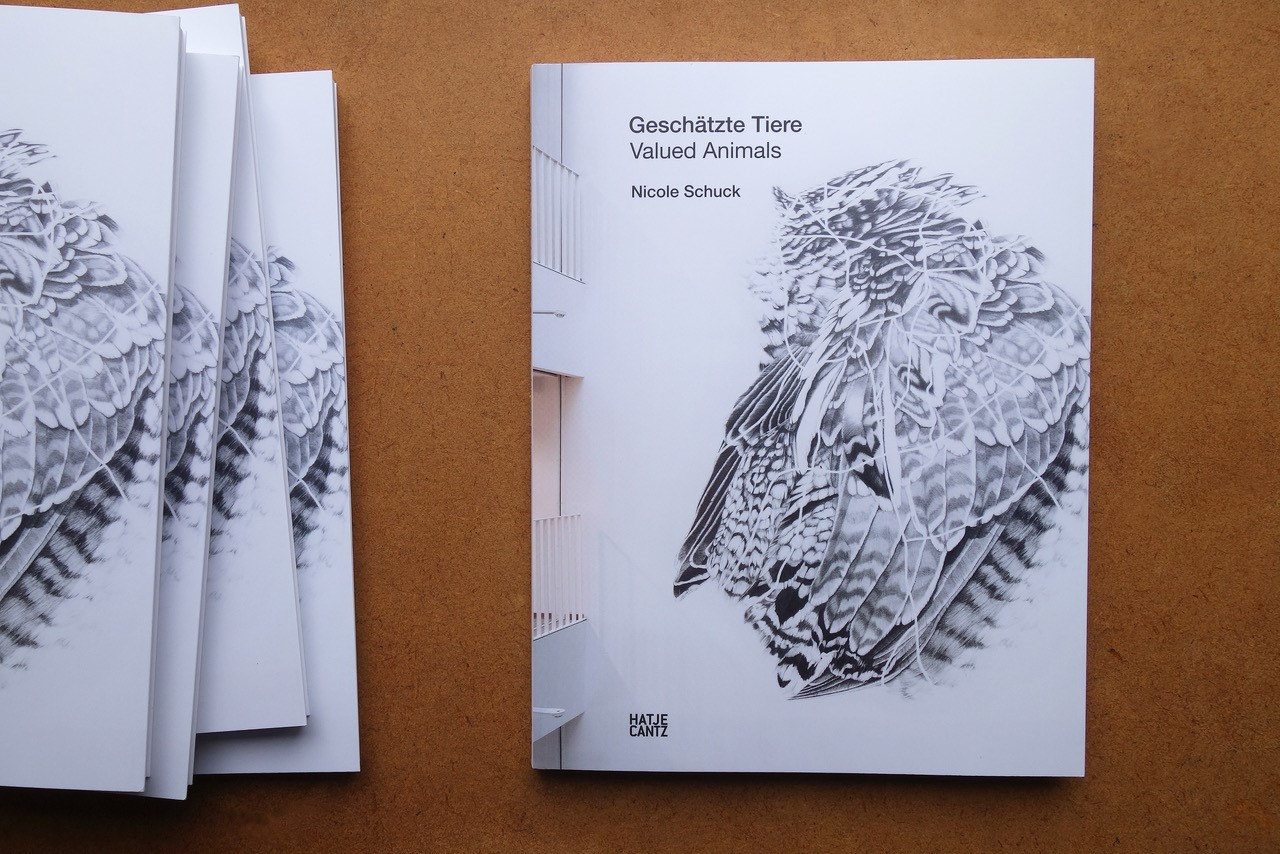
\includegraphics[width=0.9\textwidth]{img/image1.jpg}
\end{figure}

It may not be a shark in the flesh, but be prepared when you will
encounter the shark of EPFL Library, located at the Rolex Learning
Center in EPFL, Lausanne. Named \enquote{Maurice Library Security}, the
shark is an EPFL Library mascot and is used to \enquote{swim} or fly in
the Library among the students. Well, that sounds logical in a
wave-shaped building, doesn't it?

Maurice was born on April 1, 2014. His original mission was to make the
students laugh for a day. In light of the success of this April Fool's
joke, it was decided to focus the Library's next communication campaign
around the shark. The message delivered during the exam period was very
explicit: \enquote{Beware! If you don't respect Maurice's rules of
behavior, he will eat you! You've been warned!}.

As a librarian, it is sometimes unpleasant to remind library users of
the rules of good conduct. It is especially true during the exam period.
During these periods, which generally last two months a year, the spaces
are saturated and students are stressed. This can lead to readers'
inappropriate behavior and tough situations for librarians to deal with.
This is where Maurice comes in! From now on, it will no longer be the
librarians who enforce discipline, but Maurice. And the message, based
on humor rather than discipline, is getting through to the users a
little better.

The library team carried out a photo session with Maurice and printed
small posters that were placed each morning on the Library tables. The
posters showed students doing anything and everything in the library,
always with Maurice standing guard in the background. In the summer, the
library team decided to make Maurice a real star by staging him in a
series of short funny videos. Six months later, after a collaboration
with the EPFL's audiovisual department, the first videos were released
on the Library YouTube channel\footnote{\url{https://www.youtube.com/channel/UCOylyf3oGEBGF-0gWYsBWqQ}}.
Immediate success.

The years go by and, in addition to making appearances by flying in the
library during each exam period, Maurice becomes a key figure in the
library and on EPFL campus. Students parody Maurice's posters, make
caricatures of him, and the shark even gets his article in the EPFL
magazine. Maurice takes part in Vivapoly 2017 edition (EPFL annual
festival), where students can take selfies with the famous shark. Nearly
1,000 pictures were taken with Maurice during the evening. In 2018,
Maurice is the subject of a photography contest on Instagram (the photos
are visible there with the tag \#EPFLmaurice). In 2018, Maurice pulls
out all the stops during the summer exam period: a crime scene is set up
in the middle of the library. The shark, furious that some students had
reserved work seats, is said to have eaten one of them. All that remains
is a blouse stained with (fake) blood, hair, a leg, and a few clues
strewn on the floor in front of stunned students.

Six years after the first video from Maurice was posted on Youtube,
there are more than 35,000 views on videos of the shark that has become
a star on social media. But as always, fame brings its share of trouble.
As Maurice popularity grows, students realize that Maurice -- with its
image more sympathetic than threatening -- will never devour them, even
if they don't respect the rules of behavior. In other words, Maurice has
more become a communication star of the library, than an efficient way
to enforce the rules. But after all, isn't that the whole point of
having a shark in a library? Knowing that you are being watched, but not
knowing what fate has in store for you.

\emph{Maurice videos on Youtube:}\newline
\url{www.youtube.com/watch?v=zuZhUiJfb20\&list=PLPkfOHxsjx2j4WEugTP_Wo5Fj7rL7mC8P}

\emph{To know more:}\newline Conference «~La Bibliothèque communique avec ses
amis~» (french only), June 2, 2015, podcast available on
\url{https://www.youtube.com/watch?v=RR8IAkZRXeg}

%autor
\begin{center}\rule{0.5\linewidth}{0.5pt}\end{center}

\textbf{Frank Milfort} is EPFL Library communication officer since
2017 and has adopted Maurice since the first day he met him.

\end{document}
